\documentclass[10pt]{article}
\usepackage[margin=0.55in]{geometry}
\usepackage{booktabs}
\usepackage{array}
\usepackage{longtable}
\usepackage{graphicx}
\usepackage[T1]{fontenc}
\renewcommand{\arraystretch}{1.18}
\setlength{\tabcolsep}{5pt}
\newcommand{\tablecaption}[1]{\par\noindent\makebox[\textwidth][c]{\footnotesize\textbf{Table #1.}}\par\vspace{-7pt}}
\newcommand{\figurecaption}[1]{\par\noindent\makebox[\textwidth][c]{\footnotesize\textbf{Figure #1.}}\par\vspace{-7pt}}

\begin{document}

\tablecaption{1}
\begin{center}
\small
\begin{tabular}{l l r r r r}
\toprule
Dataset & Boundary configuration & Avg. segments & Train max & Val max & Base SumR \\
\midrule
ActivityNet & cosine; prom. $-1.0$; dist. 1; smooth 1 & 36 & 212 & 224 & 183.9 \\
TVR & cosine; prom. $0.2$; dist. 2; smooth 1 & 21 & 75 & 52 & 232.6 \\
Qvhighlights & cosine; prom. $1.3$; dist. 2; smooth 3; length regularization & 72 & 143 & 139 & 243.5 \\
\bottomrule
\end{tabular}
\end{center}

\tablecaption{2}
\begin{center}
\small
\begin{tabular}{l c c}
\toprule
Hyperparameter & U1 & U2 \\
\midrule
Multi-scale windows & \multicolumn{2}{c}{$\{2,4,8,16\}$} \\
Scale weights & \multicolumn{2}{c}{$\{0.4,0.3,0.2,0.1\}$} \\
Peak selection / normalization & \multicolumn{2}{c}{prominence / MAD} \\
MAD prominence & 0.4 & 0.2 \\
Minimum distance / smoothing & \multicolumn{2}{c}{1 / 1} \\
\bottomrule
\end{tabular}
\end{center}

\tablecaption{3}
\begin{center}
\small
\begin{tabular}{l l r r r r r r}
\toprule
Dataset & Setting & Avg. segments & R@1 & R@5 & R@10 & R@100 & SumR \\
\midrule
ActivityNet & Base & 36 & 15.0 & 36.4 & 49.8 & 82.8 & 183.9 \\
ActivityNet & U1 & 18 & 14.5 & 36.2 & 49.3 & 83.0 & 183.1 \\
ActivityNet & U2 & 19 & 14.5 & 36.6 & 49.7 & 82.9 & 183.7 \\
TVR & Base & 21 & 26.0 & 51.8 & 62.5 & 92.3 & 232.6 \\
TVR & U1 & 19 & 26.4 & 51.7 & 62.7 & 92.0 & 232.8 \\
TVR & U2 & 21 & 26.6 & 51.4 & 62.8 & 92.3 & 233.1 \\
Qvhighlights & Base & 72 & 26.5 & 54.9 & 66.8 & 95.3 & 243.5 \\
Qvhighlights & U1 & 139 & 24.5 & 54.3 & 67.0 & 96.7 & 242.4 \\
Qvhighlights & U2 & 149 & 26.8 & 54.5 & 67.7 & 96.5 & 245.5 \\
\bottomrule
\end{tabular}
\end{center}

\tablecaption{4}
\begin{center}
\small
\begin{tabular}{l l r r r r r}
\toprule
Dataset & Setting & R@1 & R@5 & R@10 & R@100 & SumR \\
\midrule
ActivityNet & Hard & 15.0 & 36.4 & 49.8 & 82.8 & 183.9 \\
ActivityNet & Soft & 14.5 & 36.3 & 49.6 & 83.2 & 183.6 \\
TVR & Soft & 26.0 & 51.8 & 62.5 & 92.3 & 232.6 \\
TVR & Hard & 26.9 & 51.7 & 62.3 & 92.0 & 233.0 \\
Qvhighlights & Soft & 26.5 & 54.9 & 66.8 & 95.3 & 243.5 \\
Qvhighlights & Hard & 24.2 & 53.4 & 65.5 & 96.5 & 239.6 \\
Qvhighlights & no length regularization & 25.8 & 55.2 & 66.0 & 96.1 & 243.0 \\
\bottomrule
\end{tabular}
\end{center}

\newpage
\tablecaption{5}
\begin{center}
\small
\begin{tabular}{c r r r}
\toprule
Segment:Frame & ActivityNet SumR & TVR SumR & Qvhighlights SumR \\
\midrule
0.60:0.40 & 181.8 & 228.6 & 238.3 \\
0.65:0.35 & 182.7 & 229.9 & 239.9 \\
0.70:0.30 & 183.3 & 231.2 & 241.4 \\
0.75:0.25 & 183.9 & 232.1 & 241.5 \\
0.80:0.20 & 184.7 & 232.6 & 243.5 \\
0.85:0.15 & 183.9 & 232.6 & 243.3 \\
0.90:0.10 & 184.5 & 232.8 & 243.2 \\
\bottomrule
\end{tabular}
\end{center}
\begin{center}
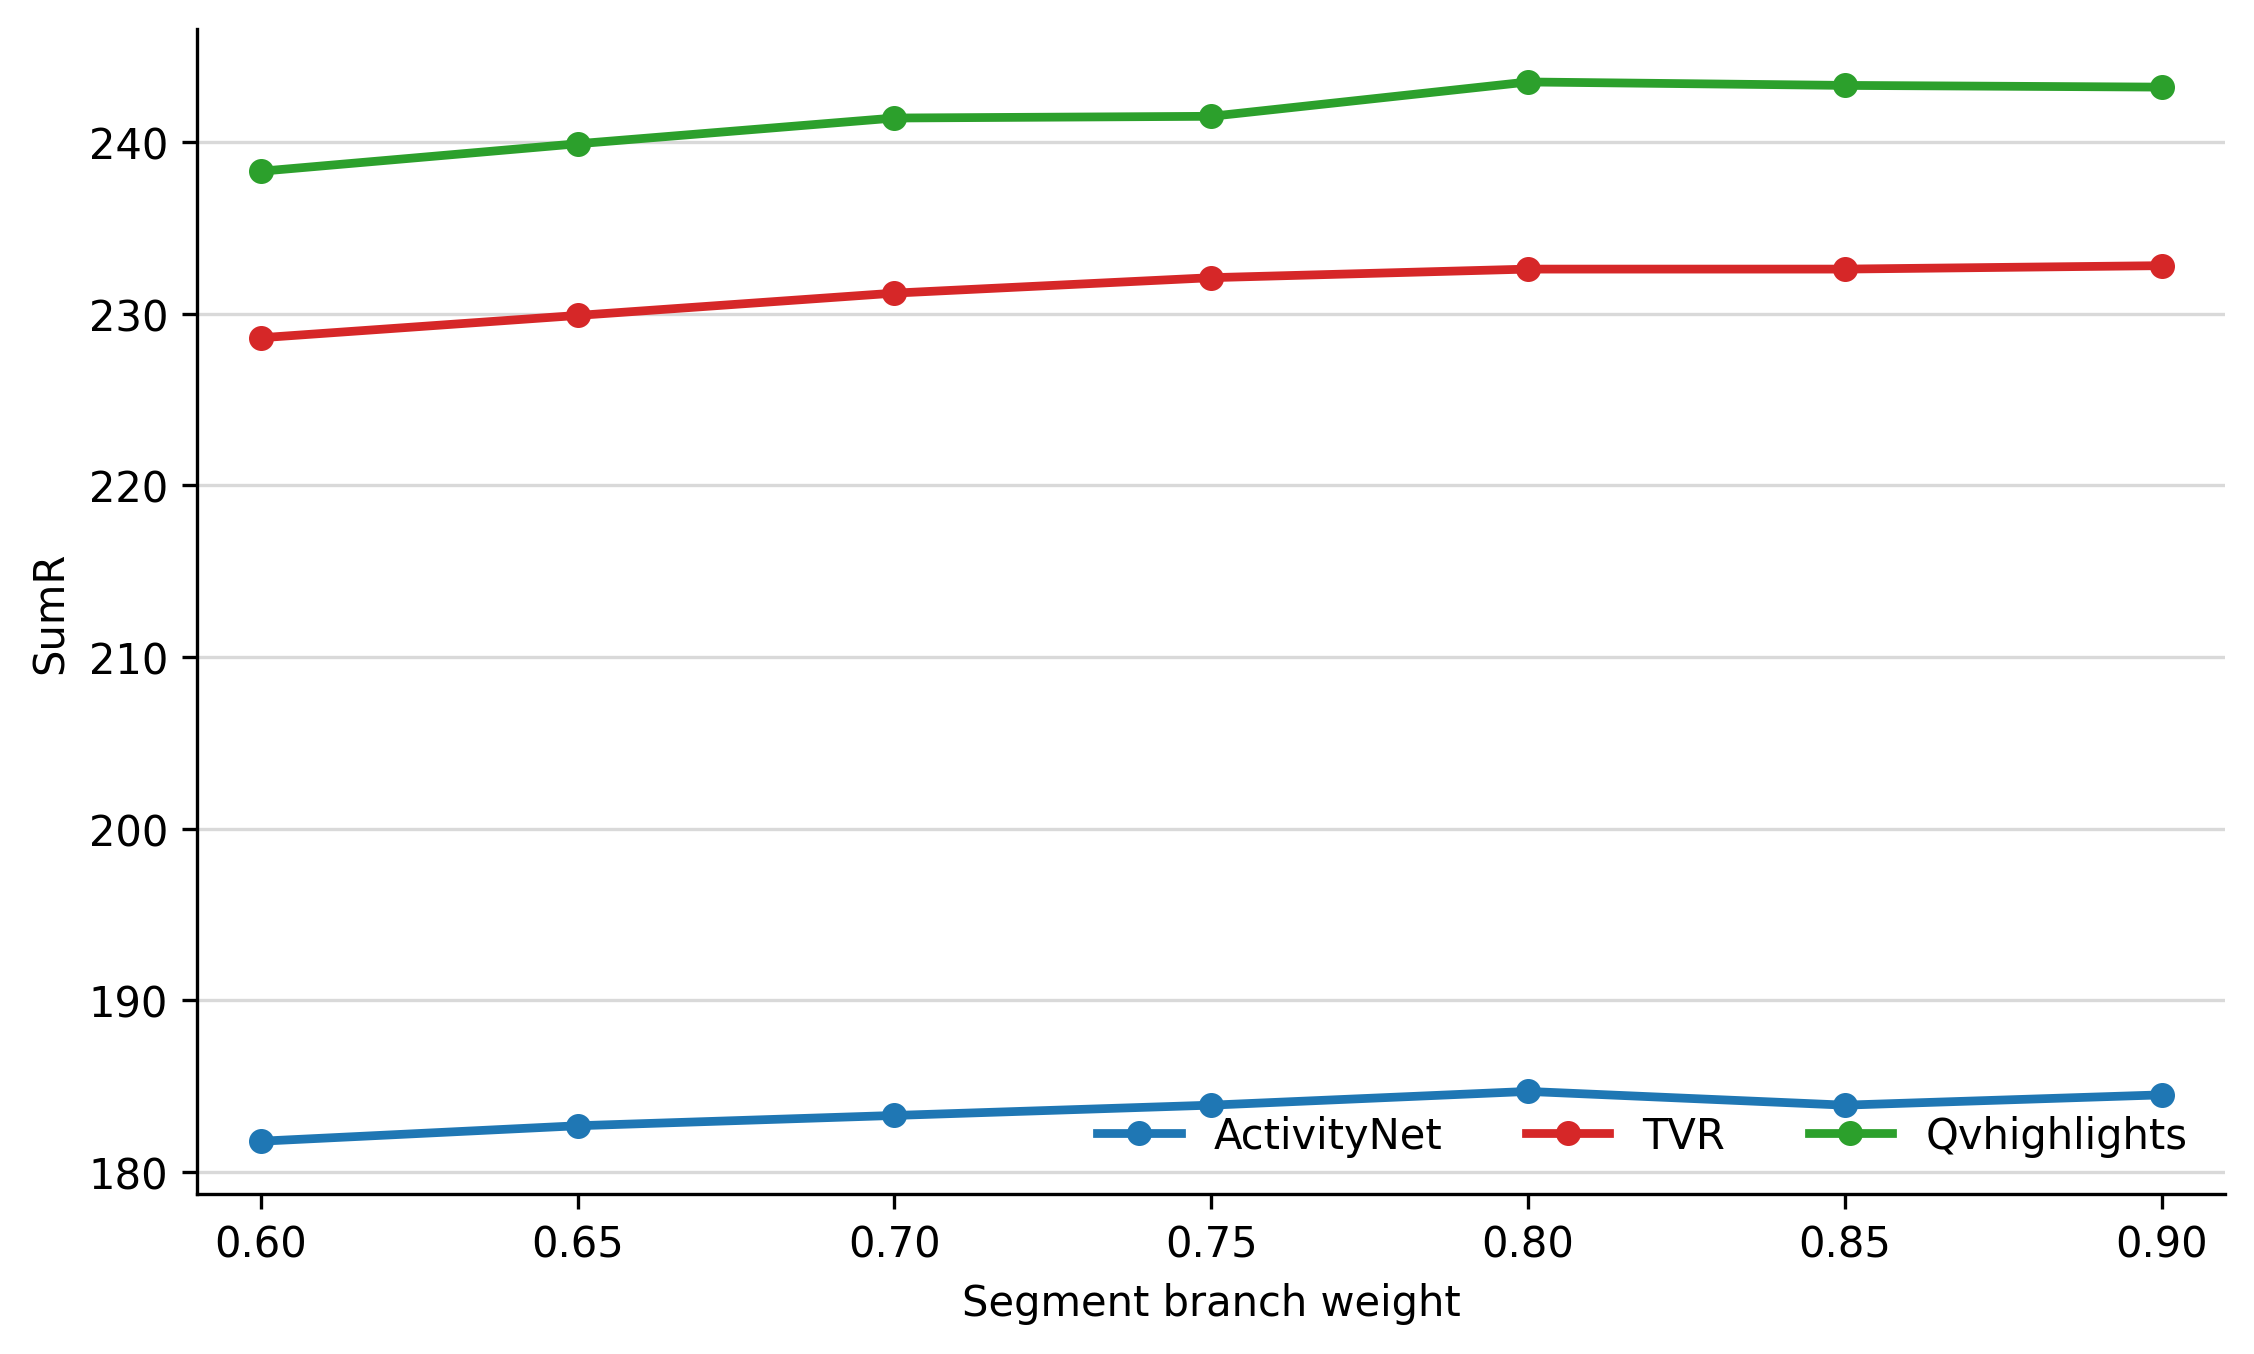
\includegraphics[width=0.65\textwidth]{rendered/fusion_sweep_sumr.png}
\end{center}
\figurecaption{1}
\vspace{10pt}
\tablecaption{6}
\begin{center}
\small
\begin{tabular}{l r}
\toprule
Dataset & Wall-clock time (s) \\
\midrule
ActivityNet & 29.981 \\
TVR & 53.653 \\
Qvhighlights & 47.766 \\
\bottomrule
\end{tabular}
\end{center}
\end{document}
